 % Pattern Info
% Pattern Info
\usetikzlibrary{patterns}
\tikzset{
	pattern size/.store in=\mcSize, 
	pattern size = 5pt,
	pattern thickness/.store in=\mcThickness, 
	pattern thickness = 0.3pt,
	pattern radius/.store in=\mcRadius, 
	pattern radius = 1pt}
\makeatletter
\pgfutil@ifundefined{pgf@pattern@name@_xfsreadb0}{
	\pgfdeclarepatternformonly[\mcThickness,\mcSize]{_xfsreadb0}
	{\pgfqpoint{0pt}{-\mcThickness}}
	{\pgfpoint{\mcSize}{\mcSize}}
	{\pgfpoint{\mcSize}{\mcSize}}
	{
		\pgfsetcolor{\tikz@pattern@color}
		\pgfsetlinewidth{\mcThickness}
		\pgfpathmoveto{\pgfqpoint{0pt}{\mcSize}}
		\pgfpathlineto{\pgfpoint{\mcSize+\mcThickness}{-\mcThickness}}
		\pgfusepath{stroke}
}}
\makeatother

% Pattern Info

\tikzset{
	pattern size/.store in=\mcSize, 
	pattern size = 5pt,
	pattern thickness/.store in=\mcThickness, 
	pattern thickness = 0.3pt,
	pattern radius/.store in=\mcRadius, 
	pattern radius = 1pt}
\makeatletter
\pgfutil@ifundefined{pgf@pattern@name@_3n2r8st5u}{
	\pgfdeclarepatternformonly[\mcThickness,\mcSize]{_3n2r8st5u}
	{\pgfqpoint{0pt}{-\mcThickness}}
	{\pgfpoint{\mcSize}{\mcSize}}
	{\pgfpoint{\mcSize}{\mcSize}}
	{
		\pgfsetcolor{\tikz@pattern@color}
		\pgfsetlinewidth{\mcThickness}
		\pgfpathmoveto{\pgfqpoint{0pt}{\mcSize}}
		\pgfpathlineto{\pgfpoint{\mcSize+\mcThickness}{-\mcThickness}}
		\pgfusepath{stroke}
}}
\makeatother
\tikzset{every picture/.style={line width=0.75pt}} %set default line width to 0.75pt
\marginnote{
	\begin{minipage}{5.5cm}
		\begin{figure}[H]\centering
			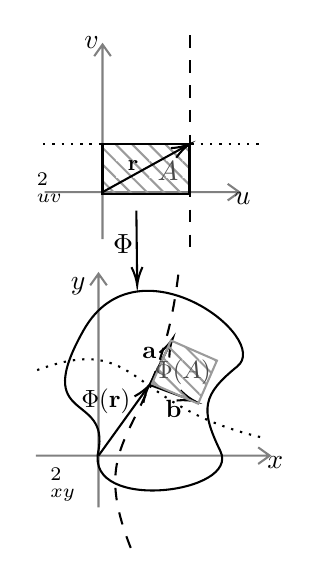
\begin{tikzpicture}[x=0.6pt,y=0.6pt,yscale=-1,xscale=1]
			%uncomment if require: \path (0,360); %set diagram left start at 0, and has height of 360
			
			%Shape: Axis 2D [id:dp6955661693387541] 
			\draw [color={rgb, 255:red, 128; green, 128; blue, 128 }  ,draw opacity=1 ] (32.75,142.91) -- (150,142.91)(67.63,54) -- (67.63,171.25) (143,137.91) -- (150,142.91) -- (143,147.91) (62.63,61) -- (67.63,54) -- (72.63,61)  ;
			%Shape: Axis 2D [id:dp02452968449879911] 
			\draw [color={rgb, 255:red, 128; green, 128; blue, 128 }  ,draw opacity=1 ] (27.54,301.61) -- (168.35,301.61)(65.21,192.01) -- (65.21,332.82) (161.35,296.61) -- (168.35,301.61) -- (161.35,306.61) (60.21,199.01) -- (65.21,192.01) -- (70.21,199.01)  ;
			%Shape: Rectangle [id:dp20948017242950956] 
			\draw  [pattern=_xfsreadb0,pattern size=6pt,pattern thickness=0.75pt,pattern radius=0pt, pattern color={rgb, 255:red, 155; green, 155; blue, 155}] (67.63,114) -- (120,114) -- (120,143.92) -- (67.63,143.92) -- cycle ;
			%Shape: Regular Polygon [id:dp69594813388231] 
			\draw   (56.23,226.04) .. controls (88.48,168.87) and (169.8,230.83) .. (148.84,247.82) .. controls (127.89,264.81) and (126.17,273.3) .. (138.56,298.79) .. controls (150.94,324.27) and (57.7,335.98) .. (65.03,299.33) .. controls (72.36,262.68) and (23.99,283.21) .. (56.23,226.04) -- cycle ;
			%Straight Lines [id:da5674798320550437] 
			\draw    (67.63,142.91) -- (118.25,114.97) ;
			\draw [shift={(120,114)}, rotate = 511.1] [color={rgb, 255:red, 0; green, 0; blue, 0 }  ][line width=0.75]    (10.93,-3.29) .. controls (6.95,-1.4) and (3.31,-0.3) .. (0,0) .. controls (3.31,0.3) and (6.95,1.4) .. (10.93,3.29)   ;
			
			%Straight Lines [id:da07583959071373081] 
			\draw    (65.21,301.61) -- (94.78,260.58) ;
			\draw [shift={(95.95,258.96)}, rotate = 485.78] [color={rgb, 255:red, 0; green, 0; blue, 0 }  ][line width=0.75]    (10.93,-3.29) .. controls (6.95,-1.4) and (3.31,-0.3) .. (0,0) .. controls (3.31,0.3) and (6.95,1.4) .. (10.93,3.29)   ;
			
			%Curve Lines [id:da4700982262625235] 
			\draw [color={rgb, 255:red, 0; green, 0; blue, 0 }  ,draw opacity=1 ] [dash pattern={on 4.5pt off 4.5pt}]  (84.62,357.17) .. controls (55.66,284.14) and (102.25,292.95) .. (113.58,189.7) ;
			
			
			%Curve Lines [id:da24363555751710253] 
			\draw [color={rgb, 255:red, 0; green, 0; blue, 0 }  ,draw opacity=1 ] [dash pattern={on 0.84pt off 2.51pt}]  (28.24,250.07) .. controls (91.99,226.58) and (80.54,272.34) .. (166.11,291.2) ;
			
			
			%Straight Lines [id:da9809152665245934] 
			\draw [color={rgb, 255:red, 0; green, 0; blue, 0 }  ,draw opacity=1 ]   (95.95,258.96) -- (108.91,233.04) ;
			\draw [shift={(109.8,231.25)}, rotate = 476.57] [color={rgb, 255:red, 0; green, 0; blue, 0 }  ,draw opacity=1 ][line width=0.75]    (10.93,-3.29) .. controls (6.95,-1.4) and (3.31,-0.3) .. (0,0) .. controls (3.31,0.3) and (6.95,1.4) .. (10.93,3.29)   ;
			
			%Straight Lines [id:da7463306935174108] 
			\draw [color={rgb, 255:red, 0; green, 0; blue, 0 }  ,draw opacity=1 ]   (95.95,258.96) -- (121.78,268.34) ;
			\draw [shift={(123.66,269.03)}, rotate = 199.98] [color={rgb, 255:red, 0; green, 0; blue, 0 }  ,draw opacity=1 ][line width=0.75]    (10.93,-3.29) .. controls (6.95,-1.4) and (3.31,-0.3) .. (0,0) .. controls (3.31,0.3) and (6.95,1.4) .. (10.93,3.29)   ;
			
			%Shape: Rectangle [id:dp6495281329284983] 
			\draw  [color={rgb, 255:red, 155; green, 155; blue, 155 }  ,draw opacity=1 ][pattern=_3n2r8st5u,pattern size=6pt,pattern thickness=0.75pt,pattern radius=0pt, pattern color={rgb, 255:red, 155; green, 155; blue, 155}] (108.8,232.25) -- (136.51,244.35) -- (125.19,270.29) -- (97.48,258.2) -- cycle ;
			%Straight Lines [id:da6330165684861724] 
			\draw  [dash pattern={on 0.84pt off 2.51pt}]  (31.85,113.93) -- (162.85,113.93) ;
			
			
			%Straight Lines [id:da6497686783668063] 
			\draw  [dash pattern={on 4.5pt off 4.5pt}]  (120.35,48.43) -- (120.35,179.43) ;
			
			
			%Straight Lines [id:da27738867786575405] 
			\draw    (88,154) -- (88.48,197) ;
			\draw [shift={(88.5,199)}, rotate = 269.36] [color={rgb, 255:red, 0; green, 0; blue, 0 }  ][line width=0.75]    (10.93,-3.29) .. controls (6.95,-1.4) and (3.31,-0.3) .. (0,0) .. controls (3.31,0.3) and (6.95,1.4) .. (10.93,3.29)   ;
			
			
			% Text Node
			\draw (152,147) node   {$u$};
			% Text Node
			\draw (61,53) node   {$v$};
			% Text Node
			\draw (171.69,305.89) node   {$x$};
			% Text Node
			\draw (52.92,199.35) node   {$y$};
			% Text Node
			\draw (86,126.67) node [scale=0.8]  {$\mathbf{r}$};
			% Text Node
			\draw (107,130) node [color={rgb, 255:red, 74; green, 74; blue, 74 }  ,opacity=1 ]  {$A$};
			% Text Node
			\draw (80,174) node   {$\Phi $};
			% Text Node
			\draw (69.62,269.04) node [scale=0.9]  {$\Phi (\mathbf{r})$};
			% Text Node
			\draw (95.81,240.04) node [scale=0.9]  {$\mathbf{a}$};
			% Text Node
			\draw (110.43,273.63) node [scale=0.9]  {$\mathbf{b}$};
			% Text Node
			\draw (116,251.27) node [scale=0.9,color={rgb, 255:red, 74; green, 74; blue, 74 }  ,opacity=1 ]  {$\Phi ( A)$};
			% Text Node
			\draw (36,140.5) node   {$\R^{2}_{uv}$};
			% Text Node
			\draw (44,319) node   {$\R^{2}_{xy}$};
			
			
			\end{tikzpicture}
			
			\caption{Mapeo del caso 2-2.}\label{ch0d4}
		\end{figure}
\end{minipage}}[-7em]